\documentclass[aspectratio=169]{beamer}

% Minimal theme
\usetheme{default}
\usecolortheme{dove}

% Remove navigation symbols
\setbeamertemplate{navigation symbols}{}
\setbeamertemplate{footline}{%
  \hfill{\large\insertframenumber\,/\,\inserttotalframenumber}\hspace{0.8em}\vspace{0.5em}%
}

% Colors
\definecolor{popblue}{RGB}{52, 101, 164}
\definecolor{sampred}{RGB}{204, 0, 0}
\definecolor{paramgreen}{RGB}{0, 140, 70}
\definecolor{lightbg}{RGB}{245, 245, 250}
\definecolor{warnred}{RGB}{180, 40, 40}
\definecolor{orange1}{RGB}{220, 120, 0}
\definecolor{violet1}{RGB}{120, 50, 160}

\setbeamercolor{frametitle}{fg=popblue}
\setbeamercolor{title}{fg=popblue}

% Packages
\usepackage{pgfplots}
\usepackage{tikz}
\usetikzlibrary{shapes, arrows.meta, positioning, calc, decorations.pathreplacing, patterns, fit}
\pgfplotsset{compat=1.18}
\usepackage{amsmath, amssymb}
\usepackage{array}
\usepackage{fontenc}

\title{Mixture of Experts}
\subtitle{Sparse Models $\cdot$ Gating $\cdot$ Load Balancing $\cdot$ Scaling}
\date{}

\begin{document}

% ============================================================
% TITLE
% ============================================================
\begin{frame}
\titlepage
\end{frame}

% ============================================================
% WHAT IS MOE?
% ============================================================
\begin{frame}
\frametitle{What is Mixture of Experts?}
\vspace{-0.2cm}
\begin{center}
\begin{tikzpicture}
  % Core idea
  \node[draw=popblue, fill=popblue!5, rounded corners=8pt, text width=11cm, align=center, inner sep=8pt, font=\small] at (0, 3) {
    \textbf{Core idea:} divide a model into separate sub-networks (\textbf{experts}),\\
    each specializing in different aspects of the input.\\[3pt]
    A \textbf{router} decides which experts to activate for each input.
  };

  % Dense vs Sparse
  \node[draw=sampred, fill=sampred!8, rounded corners=8pt, text width=4.5cm, align=center, inner sep=6pt] at (-3, 0.5) {
    \textbf{\textcolor{sampred}{Dense model}}\\[4pt]
    {\small Every input activates\\ALL parameters.}\\[4pt]
    \begin{tikzpicture}[scale=0.5]
      \fill[sampred!30] (0,0) rectangle (4,2);
      \node[font=\tiny, text=sampred] at (2,1) {100\% active};
    \end{tikzpicture}
  };

  \node[draw=paramgreen, fill=paramgreen!8, rounded corners=8pt, text width=4.5cm, align=center, inner sep=6pt] at (3.5, 0.5) {
    \textbf{\textcolor{paramgreen}{Sparse MoE model}}\\[4pt]
    {\small Each input activates only\\a SUBSET of parameters.}\\[4pt]
    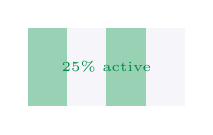
\begin{tikzpicture}[scale=0.5]
      \fill[lightbg] (0,0) rectangle (4,2);
      \fill[paramgreen!40] (0,0) rectangle (1,2);
      \fill[paramgreen!40] (2,0) rectangle (3,2);
      \node[font=\tiny, text=paramgreen] at (2,1) {25\% active};
    \end{tikzpicture}
  };

  \draw[-Stealth, very thick, paramgreen] (0, 0.5) -- (0.7, 0.5);

  % Key benefit
  \node[draw=orange1, fill=orange1!5, rounded corners=6pt, text width=11cm, align=center, inner sep=6pt, font=\small] at (0, -2) {
    \textbf{Conditional computation:} scale model capacity (total params) without\\
    proportionally increasing compute (FLOPs per token).
  };

  \node[font=\scriptsize, text=gray] at (0, -2.9) {Jacobs, Jordan, Nowlan \& Hinton, ``Adaptive Mixtures of Local Experts,'' \emph{Neural Computation}, 1991};
\end{tikzpicture}
\end{center}
\end{frame}

% ============================================================
% ARCHITECTURE
% ============================================================
\begin{frame}
\frametitle{MoE architecture}

\begin{center}
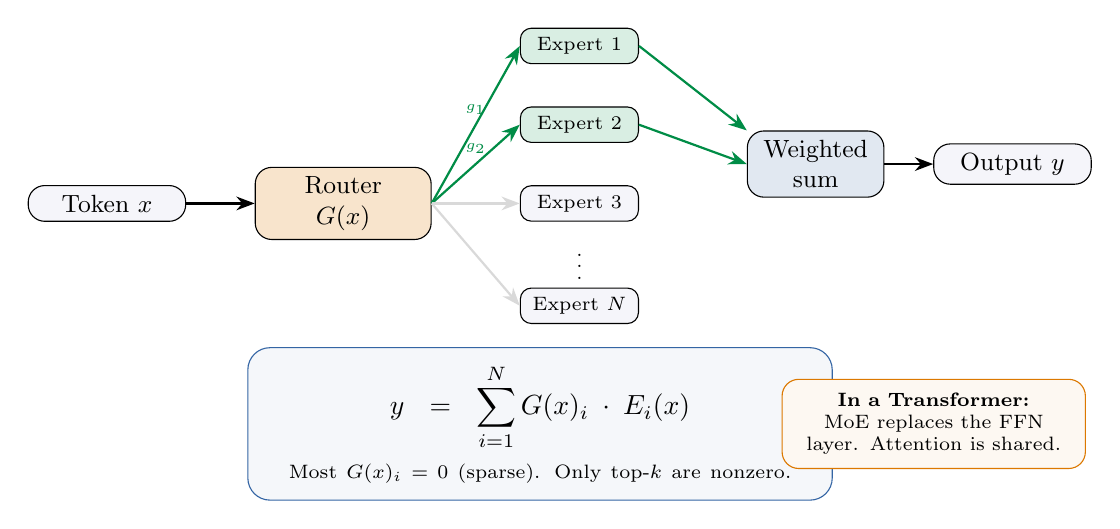
\begin{tikzpicture}
  % Input token
  \node[draw, rounded corners=6pt, fill=lightbg, font=\small, minimum width=2cm] (input) at (-5, 1) {Token $x$};

  % Router
  \node[draw, rounded corners=6pt, fill=orange1!20, font=\small, text width=2cm, align=center] (router) at (-2, 1) {Router\\$G(x)$};
  \draw[-Stealth, thick] (input) -- (router);

  % Experts
  \node[draw, rounded corners=4pt, fill=paramgreen!15, font=\scriptsize, minimum width=1.5cm] (e1) at (1, 3) {Expert 1};
  \node[draw, rounded corners=4pt, fill=paramgreen!15, font=\scriptsize, minimum width=1.5cm] (e2) at (1, 2) {Expert 2};
  \node[draw, rounded corners=4pt, fill=lightbg, font=\scriptsize, minimum width=1.5cm] (e3) at (1, 1) {Expert 3};
  \node[font=\scriptsize] at (1, 0.3) {$\vdots$};
  \node[draw, rounded corners=4pt, fill=lightbg, font=\scriptsize, minimum width=1.5cm] (en) at (1, -0.3) {Expert $N$};

  % Router arrows (only to selected experts)
  \draw[-Stealth, thick, paramgreen] (router.east) -- (e1.west) node[midway, above, font=\tiny, text=paramgreen] {$g_1$};
  \draw[-Stealth, thick, paramgreen] (router.east) -- (e2.west) node[midway, above, font=\tiny, text=paramgreen] {$g_2$};
  \draw[-Stealth, thick, gray!30] (router.east) -- (e3.west);
  \draw[-Stealth, thick, gray!30] (router.east) -- (en.west);

  % Weighted sum
  \node[draw, rounded corners=6pt, fill=popblue!15, font=\small, text width=1.5cm, align=center] (sum) at (4, 1.5) {Weighted\\sum};
  \draw[-Stealth, thick, paramgreen] (e1.east) -- (sum.north west);
  \draw[-Stealth, thick, paramgreen] (e2.east) -- (sum.west);

  % Output
  \node[draw, rounded corners=6pt, fill=lightbg, font=\small, minimum width=2cm] (output) at (6.5, 1.5) {Output $y$};
  \draw[-Stealth, thick] (sum) -- (output);

  % Formula
  \node[draw=popblue, fill=popblue!5, rounded corners=8pt, inner sep=6pt, text width=7cm, align=center] at (0.5, -1.8) {
    {\normalsize $\displaystyle y = \sum_{i=1}^{N} G(x)_i \cdot E_i(x)$}\\[4pt]
    {\scriptsize Most $G(x)_i = 0$ (sparse). Only top-$k$ are nonzero.}
  };

  % Where it sits
  \node[draw=orange1, fill=orange1!5, rounded corners=6pt, text width=3.5cm, align=center, inner sep=5pt, font=\scriptsize] at (5.5, -1.8) {
    \textbf{In a Transformer:}\\MoE replaces the FFN\\layer. Attention is shared.
  };
\end{tikzpicture}
\end{center}
\end{frame}

% ============================================================
% THE ROUTER
% ============================================================
\begin{frame}
\frametitle{The router (gating network)}
\vspace{-0.3cm}
\begin{center}
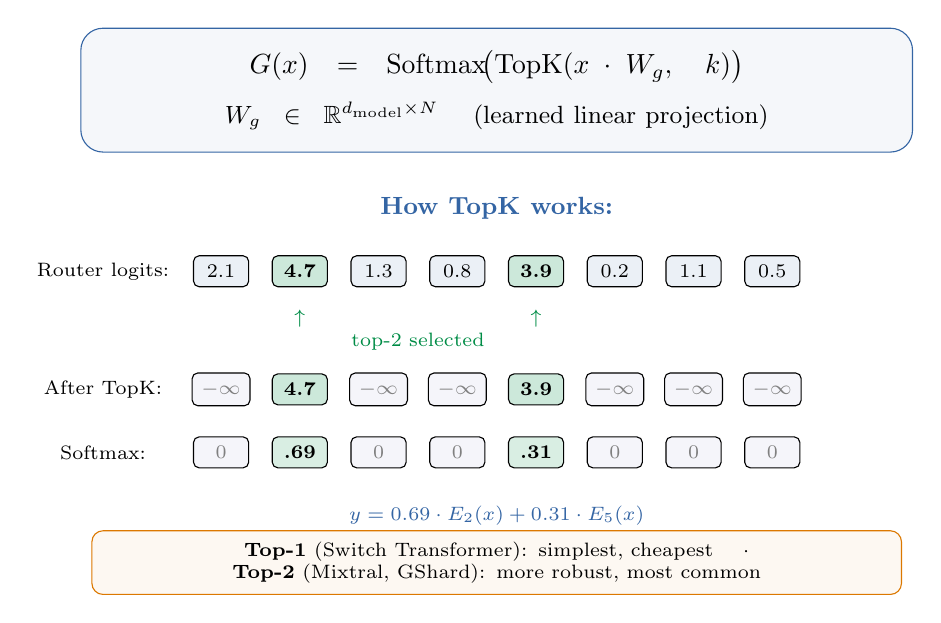
\begin{tikzpicture}
  % Router formula
  \node[draw=popblue, fill=popblue!5, rounded corners=8pt, inner sep=8pt, text width=10cm, align=center] at (0, 3) {
    {\normalsize $G(x) = \text{Softmax}\!\big(\text{TopK}(x \cdot W_g,\; k)\big)$}\\[6pt]
    {\small $W_g \in \mathbb{R}^{d_{\text{model}} \times N}$ \quad (learned linear projection)}
  };

  % Top-k explanation
  \node[font=\small\bfseries, text=popblue] at (0, 1.5) {How TopK works:};

  % Logits
  \node[font=\scriptsize] at (-5, 0.7) {Router logits:};
  \node[draw, rounded corners=2pt, fill=popblue!10, font=\scriptsize, minimum width=0.7cm] at (-3.5, 0.7) {2.1};
  \node[draw, rounded corners=2pt, fill=paramgreen!20, font=\scriptsize\bfseries, minimum width=0.7cm] at (-2.5, 0.7) {4.7};
  \node[draw, rounded corners=2pt, fill=popblue!10, font=\scriptsize, minimum width=0.7cm] at (-1.5, 0.7) {1.3};
  \node[draw, rounded corners=2pt, fill=popblue!10, font=\scriptsize, minimum width=0.7cm] at (-0.5, 0.7) {0.8};
  \node[draw, rounded corners=2pt, fill=paramgreen!20, font=\scriptsize\bfseries, minimum width=0.7cm] at (0.5, 0.7) {3.9};
  \node[draw, rounded corners=2pt, fill=popblue!10, font=\scriptsize, minimum width=0.7cm] at (1.5, 0.7) {0.2};
  \node[draw, rounded corners=2pt, fill=popblue!10, font=\scriptsize, minimum width=0.7cm] at (2.5, 0.7) {1.1};
  \node[draw, rounded corners=2pt, fill=popblue!10, font=\scriptsize, minimum width=0.7cm] at (3.5, 0.7) {0.5};

  \node[font=\scriptsize, text=paramgreen] at (-2.5, 0.1) {$\uparrow$};
  \node[font=\scriptsize, text=paramgreen] at (0.5, 0.1) {$\uparrow$};
  \node[font=\scriptsize, text=paramgreen] at (-1, -0.2) {top-2 selected};

  % After masking
  \node[font=\scriptsize] at (-5, -0.8) {After TopK:};
  \node[draw, rounded corners=2pt, fill=lightbg, font=\scriptsize, minimum width=0.7cm, text=gray] at (-3.5, -0.8) {$-\infty$};
  \node[draw, rounded corners=2pt, fill=paramgreen!20, font=\scriptsize\bfseries, minimum width=0.7cm] at (-2.5, -0.8) {4.7};
  \node[draw, rounded corners=2pt, fill=lightbg, font=\scriptsize, minimum width=0.7cm, text=gray] at (-1.5, -0.8) {$-\infty$};
  \node[draw, rounded corners=2pt, fill=lightbg, font=\scriptsize, minimum width=0.7cm, text=gray] at (-0.5, -0.8) {$-\infty$};
  \node[draw, rounded corners=2pt, fill=paramgreen!20, font=\scriptsize\bfseries, minimum width=0.7cm] at (0.5, -0.8) {3.9};
  \node[draw, rounded corners=2pt, fill=lightbg, font=\scriptsize, minimum width=0.7cm, text=gray] at (1.5, -0.8) {$-\infty$};
  \node[draw, rounded corners=2pt, fill=lightbg, font=\scriptsize, minimum width=0.7cm, text=gray] at (2.5, -0.8) {$-\infty$};
  \node[draw, rounded corners=2pt, fill=lightbg, font=\scriptsize, minimum width=0.7cm, text=gray] at (3.5, -0.8) {$-\infty$};

  % Softmax result
  \node[font=\scriptsize] at (-5, -1.6) {Softmax:};
  \node[draw, rounded corners=2pt, fill=lightbg, font=\scriptsize, minimum width=0.7cm, text=gray] at (-3.5, -1.6) {0};
  \node[draw, rounded corners=2pt, fill=paramgreen!15, font=\scriptsize\bfseries, minimum width=0.7cm] at (-2.5, -1.6) {.69};
  \node[draw, rounded corners=2pt, fill=lightbg, font=\scriptsize, minimum width=0.7cm, text=gray] at (-1.5, -1.6) {0};
  \node[draw, rounded corners=2pt, fill=lightbg, font=\scriptsize, minimum width=0.7cm, text=gray] at (-0.5, -1.6) {0};
  \node[draw, rounded corners=2pt, fill=paramgreen!15, font=\scriptsize\bfseries, minimum width=0.7cm] at (0.5, -1.6) {.31};
  \node[draw, rounded corners=2pt, fill=lightbg, font=\scriptsize, minimum width=0.7cm, text=gray] at (1.5, -1.6) {0};
  \node[draw, rounded corners=2pt, fill=lightbg, font=\scriptsize, minimum width=0.7cm, text=gray] at (2.5, -1.6) {0};
  \node[draw, rounded corners=2pt, fill=lightbg, font=\scriptsize, minimum width=0.7cm, text=gray] at (3.5, -1.6) {0};

  % output
  \node[font=\scriptsize, text=popblue] at (0, -2.4) {$y = 0.69 \cdot E_2(x) + 0.31 \cdot E_5(x)$};

  % Routing options
  \node[draw=orange1, fill=orange1!5, rounded corners=4pt, text width=10cm, align=center, inner sep=4pt, font=\scriptsize] at (0, -3.0) {
    \textbf{Top-1} (Switch Transformer): simplest, cheapest \quad $\cdot$ \quad
    \textbf{Top-2} (Mixtral, GShard): more robust, most common
  };
\end{tikzpicture}
\end{center}
\end{frame}

% ============================================================
% NOISY GATING
% ============================================================
\begin{frame}
\frametitle{Noisy top-$k$ gating}

\begin{center}
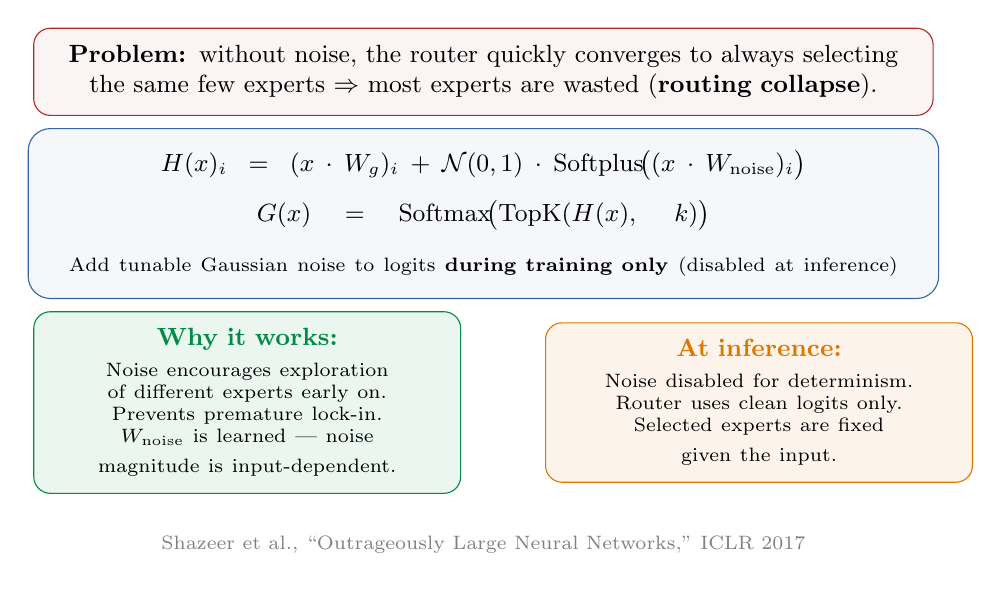
\begin{tikzpicture}
  % Problem
  \node[draw=warnred, fill=warnred!5, rounded corners=6pt, text width=11cm, align=center, inner sep=6pt, font=\small] at (0, 3) {
    \textbf{Problem:} without noise, the router quickly converges to always selecting\\
    the same few experts $\Rightarrow$ most experts are wasted (\textbf{routing collapse}).
  };

  % Solution
  \node[draw=popblue, fill=popblue!5, rounded corners=8pt, inner sep=8pt, text width=11cm, align=center] at (0, 1.2) {
    {\small $H(x)_i = (x \cdot W_g)_i + \mathcal{N}(0,1) \cdot \text{Softplus}\!\big((x \cdot W_{\text{noise}})_i\big)$}\\[6pt]
    {\small $G(x) = \text{Softmax}\!\big(\text{TopK}(H(x),\; k)\big)$}\\[6pt]
    {\scriptsize Add tunable Gaussian noise to logits \textbf{during training only} (disabled at inference)}
  };

  % Why it works
  \node[draw=paramgreen, fill=paramgreen!8, rounded corners=6pt, text width=5cm, align=center, inner sep=6pt, font=\small] at (-3, -1.2) {
    \textbf{\textcolor{paramgreen}{Why it works:}}\\[3pt]
    {\scriptsize Noise encourages exploration\\of different experts early on.\\Prevents premature lock-in.\\$W_{\text{noise}}$ is learned --- noise\\magnitude is input-dependent.}
  };

  \node[draw=orange1, fill=orange1!8, rounded corners=6pt, text width=5cm, align=center, inner sep=6pt, font=\small] at (3.5, -1.2) {
    \textbf{\textcolor{orange1}{At inference:}}\\[3pt]
    {\scriptsize Noise disabled for determinism.\\Router uses clean logits only.\\Selected experts are fixed\\given the input.}
  };

  \node[font=\scriptsize, text=gray] at (0, -3) {Shazeer et al., ``Outrageously Large Neural Networks,'' ICLR 2017};
\end{tikzpicture}
\end{center}
\end{frame}

% ============================================================
% LOAD BALANCING
% ============================================================
\begin{frame}
\frametitle{Load balancing}

\vspace{-0.3cm}
\begin{center}
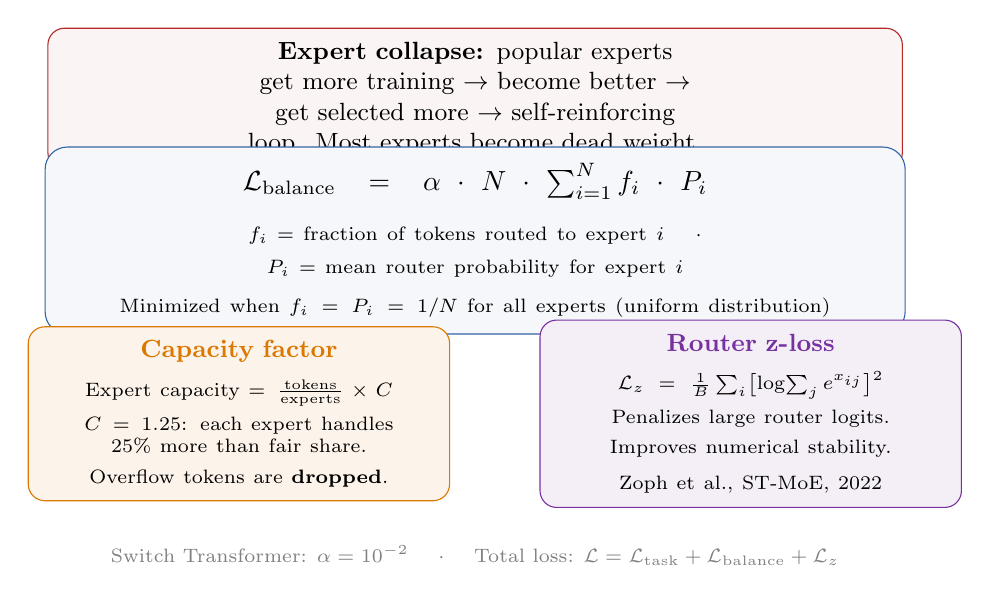
\begin{tikzpicture}
  % Expert collapse
  \node[draw=warnred, fill=warnred!5, rounded corners=6pt, text width=10.5cm, align=center, inner sep=5pt, font=\small] at (0, 2.8) {
    \textbf{Expert collapse:} popular experts get more training $\to$ become better $\to$\\
    get selected more $\to$ self-reinforcing loop. Most experts become dead weight.
  };

  % Auxiliary loss
  \node[draw=popblue, fill=popblue!5, rounded corners=8pt, inner sep=6pt, text width=10.5cm, align=center] at (0, 1) {
    {\normalsize $\mathcal{L}_{\text{balance}} = \alpha \cdot N \cdot \sum_{i=1}^{N} f_i \cdot P_i$}\\[6pt]
    {\scriptsize $f_i$ = fraction of tokens routed to expert $i$ \quad $\cdot$ \quad $P_i$ = mean router probability for expert $i$}\\[2pt]
    {\scriptsize Minimized when $f_i = P_i = 1/N$ for all experts (uniform distribution)}
  };

  % Capacity factor
  \node[draw=orange1, fill=orange1!8, rounded corners=6pt, text width=5cm, align=center, inner sep=5pt, font=\small] at (-3, -1.2) {
    \textbf{\textcolor{orange1}{Capacity factor}}\\[3pt]
    {\scriptsize Expert capacity $= \frac{\text{tokens}}{\text{experts}} \times C$}\\[3pt]
    {\scriptsize $C = 1.25$: each expert handles\\25\% more than fair share.\\Overflow tokens are \textbf{dropped}.}
  };

  % Router z-loss
  \node[draw=violet1, fill=violet1!8, rounded corners=6pt, text width=5cm, align=center, inner sep=5pt, font=\small] at (3.5, -1.2) {
    \textbf{\textcolor{violet1}{Router z-loss}}\\[3pt]
    {\scriptsize $\mathcal{L}_z = \frac{1}{B}\sum_i \!\big[\!\log\!\sum_j e^{x_{ij}}\big]^2$}\\[3pt]
    {\scriptsize Penalizes large router logits.\\Improves numerical stability.}\\[2pt]
    {\scriptsize Zoph et al., ST-MoE, 2022}
  };

  % Typical alpha
  \node[font=\scriptsize, text=gray] at (0, -3) {
    Switch Transformer: $\alpha = 10^{-2}$ \quad $\cdot$ \quad Total loss: $\mathcal{L} = \mathcal{L}_{\text{task}} + \mathcal{L}_{\text{balance}} + \mathcal{L}_z$
  };
\end{tikzpicture}
\end{center}
\end{frame}

% ============================================================
% LANDMARK PAPERS
% ============================================================
\begin{frame}
\frametitle{Landmark MoE papers}

\vspace{-0.2cm}
\begin{center}
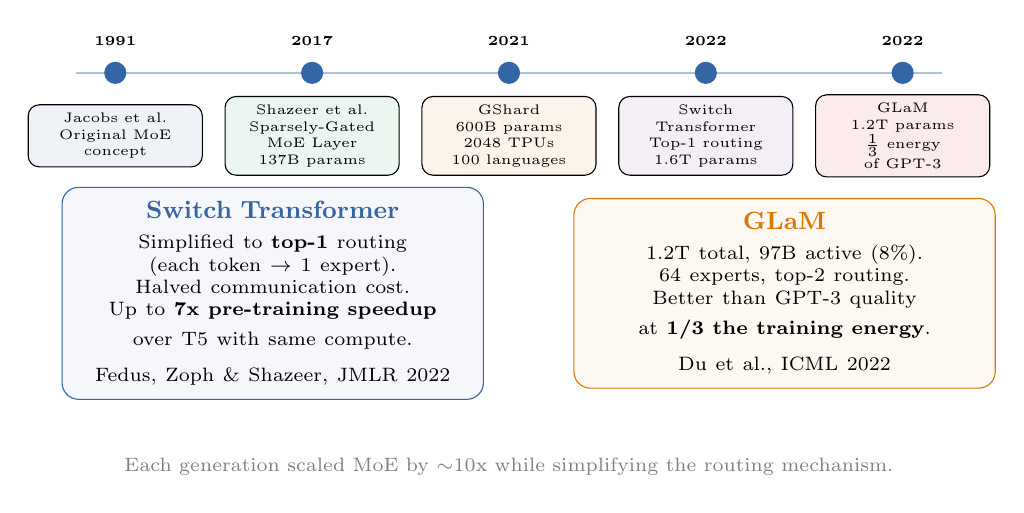
\begin{tikzpicture}
  % Timeline
  \draw[thick, popblue!40] (-5.5, 2.5) -- (5.5, 2.5);
  \fill[popblue] (-5, 2.5) circle (4pt);
  \fill[popblue] (-2.5, 2.5) circle (4pt);
  \fill[popblue] (0, 2.5) circle (4pt);
  \fill[popblue] (2.5, 2.5) circle (4pt);
  \fill[popblue] (5, 2.5) circle (4pt);

  \node[font=\tiny\bfseries] at (-5, 2.9) {1991};
  \node[font=\tiny\bfseries] at (-2.5, 2.9) {2017};
  \node[font=\tiny\bfseries] at (0, 2.9) {2021};
  \node[font=\tiny\bfseries] at (2.5, 2.9) {2022};
  \node[font=\tiny\bfseries] at (5, 2.9) {2022};

  % Paper cards
  \node[draw, rounded corners=4pt, fill=popblue!8, text width=2cm, align=center, inner sep=3pt, font=\tiny] at (-5, 1.7) {Jacobs et al.\\Original MoE\\concept};

  \node[draw, rounded corners=4pt, fill=paramgreen!8, text width=2cm, align=center, inner sep=3pt, font=\tiny] at (-2.5, 1.7) {Shazeer et al.\\Sparsely-Gated\\MoE Layer\\137B params};

  \node[draw, rounded corners=4pt, fill=orange1!8, text width=2cm, align=center, inner sep=3pt, font=\tiny] at (0, 1.7) {GShard\\600B params\\2048 TPUs\\100 languages};

  \node[draw, rounded corners=4pt, fill=violet1!8, text width=2cm, align=center, inner sep=3pt, font=\tiny] at (2.5, 1.7) {Switch\\Transformer\\Top-1 routing\\1.6T params};

  \node[draw, rounded corners=4pt, fill=sampred!8, text width=2cm, align=center, inner sep=3pt, font=\tiny] at (5, 1.7) {GLaM\\1.2T params\\$\frac{1}{3}$ energy\\of GPT-3};

  % Switch Transformer details
  \node[draw=popblue, fill=popblue!5, rounded corners=6pt, text width=5cm, align=center, inner sep=5pt, font=\small] at (-3, -0.3) {
    \textbf{\textcolor{popblue}{Switch Transformer}}\\[3pt]
    {\scriptsize Simplified to \textbf{top-1} routing\\(each token $\to$ 1 expert).\\Halved communication cost.\\Up to \textbf{7x pre-training speedup}\\over T5 with same compute.}\\[2pt]
    {\scriptsize Fedus, Zoph \& Shazeer, JMLR 2022}
  };

  % GLaM details
  \node[draw=orange1, fill=orange1!5, rounded corners=6pt, text width=5cm, align=center, inner sep=5pt, font=\small] at (3.5, -0.3) {
    \textbf{\textcolor{orange1}{GLaM}}\\[3pt]
    {\scriptsize 1.2T total, 97B active (8\%).\\64 experts, top-2 routing.\\Better than GPT-3 quality\\at \textbf{1/3 the training energy}.}\\[2pt]
    {\scriptsize Du et al., ICML 2022}
  };

  % Bottom
  \node[font=\scriptsize, text=gray, text width=10cm, align=center] at (0, -2.5) {
    Each generation scaled MoE by $\sim$10x while simplifying the routing mechanism.
  };
\end{tikzpicture}
\end{center}
\end{frame}

% ============================================================
% MODERN MOE MODELS
% ============================================================
\begin{frame}
\frametitle{Modern MoE models}

\vspace{-0.2cm}
\renewcommand{\arraystretch}{1.3}
\begin{center}
{\small
\begin{tabular}{>{\bfseries}l r r c c l}
  \textbf{Model} & \textbf{Total} & \textbf{Active} & \textbf{Experts} & \textbf{Top-$k$} & \textbf{Notes} \\
  \hline
  \textcolor{popblue}{Mixtral 8x7B} & 46.7B & 12.9B & 8 & 2 & Beats LLaMA2-70B \\[1pt]
  \textcolor{popblue}{Mixtral 8x22B} & 176B & 44B & 8 & 2 & Larger variant \\[1pt]
  \textcolor{paramgreen}{DeepSeek-V2} & 236B & 21B & 160+2 & 6+2 & Fine-grained MoE \\[1pt]
  \textcolor{paramgreen}{DeepSeek-V3} & 671B & 37B & 256+1 & 8+1 & \$5.5M training cost \\[1pt]
  \textcolor{orange1}{DBRX} & 132B & 36B & 16 & 4 & Fine-grained, 16-choose-4 \\[1pt]
  \textcolor{violet1}{Grok-1} & 314B & $\sim$79B & 8 & 2 & Open-source (xAI) \\[1pt]
  \textcolor{sampred}{Arctic} & 480B & 17B & 128 & 2 & Dense+MoE hybrid \\
  \hline
\end{tabular}
}
\end{center}

\vspace{0.2cm}
\begin{center}

\begin{tikzpicture}
  \node[draw=popblue, fill=popblue!5, rounded corners=6pt, text width=10.5cm, align=center, inner sep=6pt, font=\small] at (0, 0) {
    As of 2025, nearly all frontier models use MoE: GPT-4 (rumored 16 experts),\\
    Gemini 1.5, DeepSeek-R1, Qwen3-235B. Dense-only models are the exception.
  };
\end{tikzpicture}
\end{center}
\end{frame}

% ============================================================
% MOE VS DENSE
% ============================================================
\begin{frame}
\frametitle{MoE vs.\ dense models}
\vspace{-0.3cm}
\begin{center}
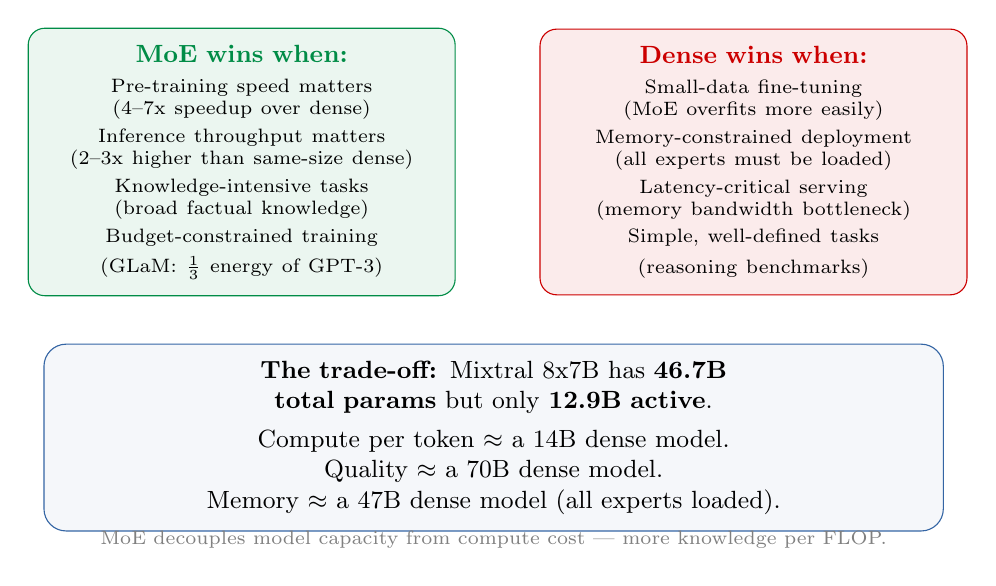
\begin{tikzpicture}
  % MoE wins
  \node[draw=paramgreen, fill=paramgreen!8, rounded corners=6pt, text width=5cm, align=center, inner sep=6pt, font=\small] at (-3, 2) {
    \textbf{\textcolor{paramgreen}{MoE wins when:}}\\[3pt]
    {\scriptsize Pre-training speed matters\\(4--7x speedup over dense)\\[2pt]
    Inference throughput matters\\(2--3x higher than same-size dense)\\[2pt]
    Knowledge-intensive tasks\\(broad factual knowledge)\\[2pt]
    Budget-constrained training\\(GLaM: $\frac{1}{3}$ energy of GPT-3)}
  };

  % Dense wins
  \node[draw=sampred, fill=sampred!8, rounded corners=6pt, text width=5cm, align=center, inner sep=6pt, font=\small] at (3.5, 2) {
    \textbf{\textcolor{sampred}{Dense wins when:}}\\[3pt]
    {\scriptsize Small-data fine-tuning\\(MoE overfits more easily)\\[2pt]
    Memory-constrained deployment\\(all experts must be loaded)\\[2pt]
    Latency-critical serving\\(memory bandwidth bottleneck)\\[2pt]
    Simple, well-defined tasks\\(reasoning benchmarks)}
  };

  % Key comparison
  \node[draw=popblue, fill=popblue!5, rounded corners=8pt, text width=11cm, align=center, inner sep=6pt, font=\small] at (0.2, -1.5) {
    \textbf{The trade-off:} Mixtral 8x7B has \textbf{46.7B total params} but only \textbf{12.9B active}.\\[3pt]
    Compute per token $\approx$ a 14B dense model.\\
    Quality $\approx$ a 70B dense model.\\
    Memory $\approx$ a 47B dense model (all experts loaded).
  };

  % Key insight
  \node[font=\scriptsize, text=gray, text width=10cm, align=center] at (0.2, -2.8) {
    MoE decouples model capacity from compute cost --- more knowledge per FLOP.
  };
\end{tikzpicture}
\end{center}
\end{frame}

% ============================================================
% GATING MECHANISMS COMPARED
% ============================================================
\begin{frame}
\frametitle{Gating mechanisms compared}

\vspace{-0.2cm}
\renewcommand{\arraystretch}{1.3}
\begin{center}
{\small
\begin{tabular}{>{\bfseries}l l l l}
  \textbf{Method} & \textbf{Who chooses?} & \textbf{Balance} & \textbf{Used by} \\
  \hline
  \textcolor{popblue}{Top-1} & Token $\to$ 1 expert & Aux loss & Switch Transformer \\[2pt]
  \textcolor{paramgreen}{Top-2} & Token $\to$ 2 experts & Aux loss & Mixtral, GShard \\[2pt]
  \textcolor{orange1}{Expert Choice} & Expert $\to$ top-$k$ tokens & Perfect & Google (2022) \\[2pt]
  \textcolor{violet1}{Soft MoE} & Weighted avg (all) & N/A & Puigcerver (2024) \\[2pt]
  \textcolor{sampred}{Hash routing} & Hash function & Random & Roller et al.\ (2021) \\
  \hline
\end{tabular}
}
\end{center}

\vspace{0.2cm}
\begin{center}
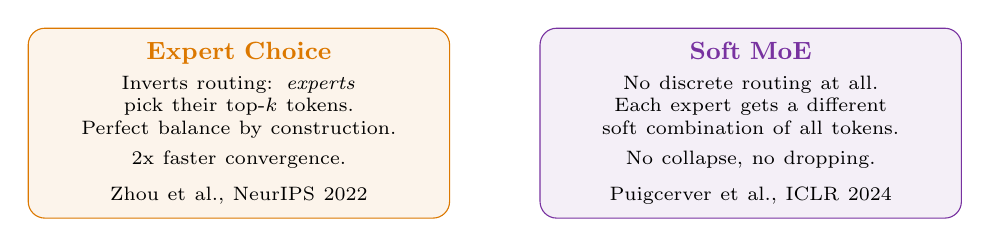
\begin{tikzpicture}
  \node[draw=orange1, fill=orange1!8, rounded corners=6pt, text width=5cm, align=center, inner sep=5pt, font=\small] at (-3, 0) {
    \textbf{\textcolor{orange1}{Expert Choice}}\\[3pt]
    {\scriptsize Inverts routing: \emph{experts}\\pick their top-$k$ tokens.\\Perfect balance by construction.\\2x faster convergence.}\\[2pt]
    {\scriptsize Zhou et al., NeurIPS 2022}
  };

  \node[draw=violet1, fill=violet1!8, rounded corners=6pt, text width=5cm, align=center, inner sep=5pt, font=\small] at (3.5, 0) {
    \textbf{\textcolor{violet1}{Soft MoE}}\\[3pt]
    {\scriptsize No discrete routing at all.\\Each expert gets a different\\soft combination of all tokens.\\No collapse, no dropping.}\\[2pt]
    {\scriptsize Puigcerver et al., ICLR 2024}
  };
\end{tikzpicture}
\end{center}
\end{frame}

% ============================================================
% EXPERT SPECIALIZATION
% ============================================================
\begin{frame}
\frametitle{What do experts learn?}

\begin{center}
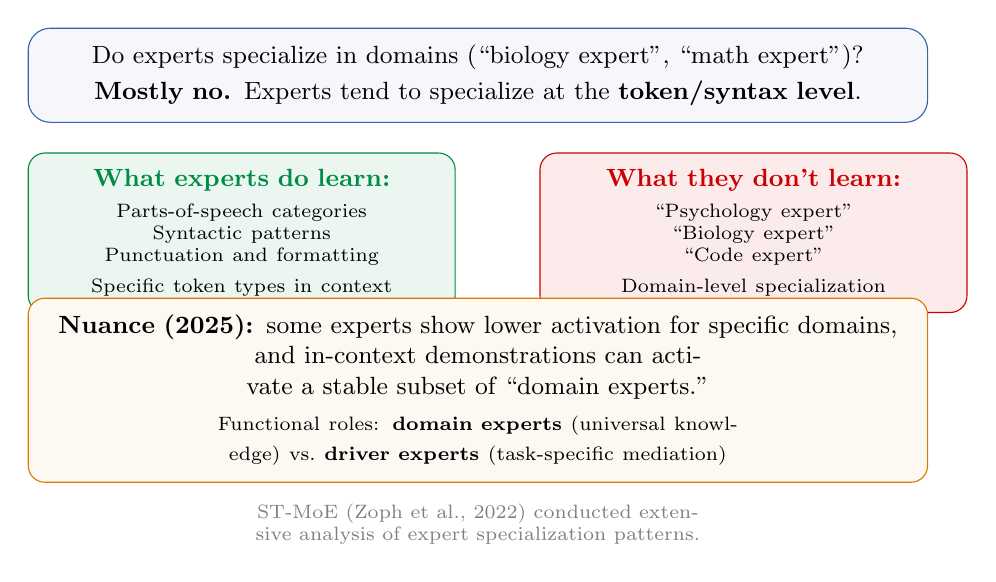
\begin{tikzpicture}
  % Question
  \node[draw=popblue, fill=popblue!5, rounded corners=8pt, text width=11cm, align=center, inner sep=6pt, font=\small] at (0, 3) {
    Do experts specialize in domains (``biology expert'', ``math expert'')?\\[2pt]
    \textbf{Mostly no.} Experts tend to specialize at the \textbf{token/syntax level}.
  };

  % What they learn
  \node[draw=paramgreen, fill=paramgreen!8, rounded corners=6pt, text width=5cm, align=center, inner sep=6pt, font=\small] at (-3, 1) {
    \textbf{\textcolor{paramgreen}{What experts do learn:}}\\[3pt]
    {\scriptsize Parts-of-speech categories\\Syntactic patterns\\Punctuation and formatting\\Specific token types in context}
  };

  \node[draw=sampred, fill=sampred!8, rounded corners=6pt, text width=5cm, align=center, inner sep=6pt, font=\small] at (3.5, 1) {
    \textbf{\textcolor{sampred}{What they don't learn:}}\\[3pt]
    {\scriptsize ``Psychology expert''\\``Biology expert''\\``Code expert''\\Domain-level specialization}
  };

  % Nuance
  \node[draw=orange1, fill=orange1!5, rounded corners=6pt, text width=11cm, align=center, inner sep=6pt, font=\small] at (0, -1) {
    \textbf{Nuance (2025):} some experts show lower activation for specific domains,\\
    and in-context demonstrations can activate a stable subset of ``domain experts.''\\[2pt]
    {\scriptsize Functional roles: \textbf{domain experts} (universal knowledge) vs.\ \textbf{driver experts} (task-specific mediation)}
  };

  % Practical implication
  \node[font=\scriptsize, text=gray, text width=10cm, align=center] at (0, -2.7) {
    ST-MoE (Zoph et al., 2022) conducted extensive analysis of expert specialization patterns.
  };
\end{tikzpicture}
\end{center}
\end{frame}

% ============================================================
% FINE-GRAINED MOE
% ============================================================
\begin{frame}
\frametitle{Fine-grained MoE (DeepSeek)}

\begin{center}
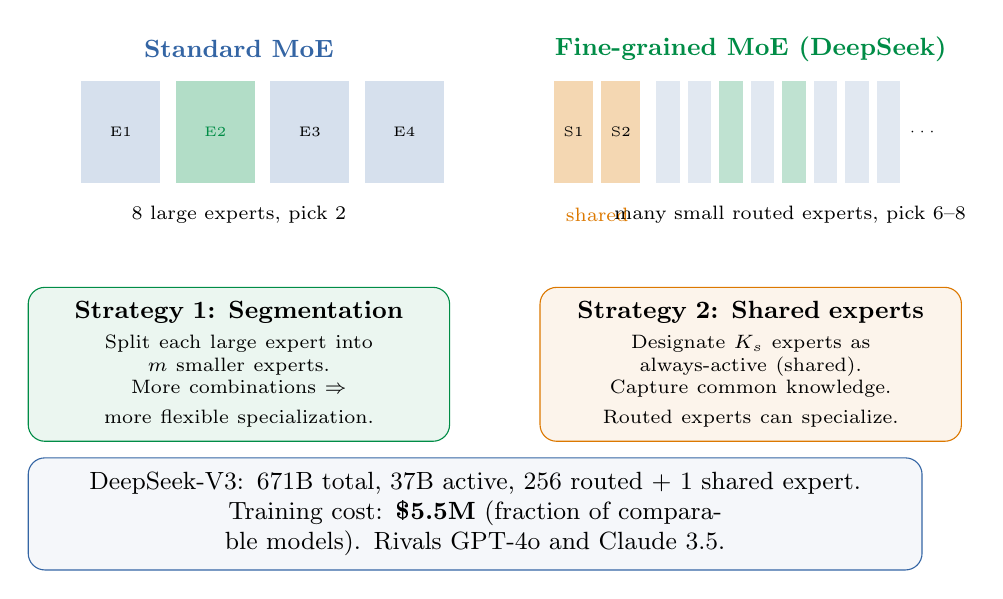
\begin{tikzpicture}
  % Standard MoE
  \node[font=\small\bfseries, text=popblue] at (-3, 3.2) {Standard MoE};

  \fill[popblue!20] (-5, 1.5) rectangle (-4, 2.8);
  \fill[paramgreen!30] (-3.8, 1.5) rectangle (-2.8, 2.8);
  \fill[popblue!20] (-2.6, 1.5) rectangle (-1.6, 2.8);
  \fill[popblue!20] (-1.4, 1.5) rectangle (-0.4, 2.8);

  \node[font=\tiny] at (-4.5, 2.15) {E1};
  \node[font=\tiny, text=paramgreen] at (-3.3, 2.15) {E2};
  \node[font=\tiny] at (-2.1, 2.15) {E3};
  \node[font=\tiny] at (-0.9, 2.15) {E4};

  \node[font=\scriptsize] at (-3, 1.1) {8 large experts, pick 2};

  % Fine-grained MoE
  \node[font=\small\bfseries, text=paramgreen] at (3.5, 3.2) {Fine-grained MoE (DeepSeek)};

  % Shared experts
  \fill[orange1!30] (1, 1.5) rectangle (1.5, 2.8);
  \fill[orange1!30] (1.6, 1.5) rectangle (2.1, 2.8);
  \node[font=\tiny] at (1.25, 2.15) {S1};
  \node[font=\tiny] at (1.85, 2.15) {S2};

  % Routed experts (many small)
  \fill[popblue!15] (2.3, 1.5) rectangle (2.6, 2.8);
  \fill[popblue!15] (2.7, 1.5) rectangle (3, 2.8);
  \fill[paramgreen!25] (3.1, 1.5) rectangle (3.4, 2.8);
  \fill[popblue!15] (3.5, 1.5) rectangle (3.8, 2.8);
  \fill[paramgreen!25] (3.9, 1.5) rectangle (4.2, 2.8);
  \fill[popblue!15] (4.3, 1.5) rectangle (4.6, 2.8);
  \fill[popblue!15] (4.7, 1.5) rectangle (5, 2.8);
  \fill[popblue!15] (5.1, 1.5) rectangle (5.4, 2.8);
  \node[font=\tiny] at (5.7, 2.15) {$\cdots$};

  \node[font=\scriptsize, text=orange1] at (1.55, 1.1) {shared};
  \node[font=\scriptsize] at (4, 1.1) {many small routed experts, pick 6--8};

  % Two strategies
  \node[draw=paramgreen, fill=paramgreen!8, rounded corners=6pt, text width=5cm, align=center, inner sep=5pt, font=\small] at (-3, -0.8) {
    \textbf{Strategy 1: Segmentation}\\[3pt]
    {\scriptsize Split each large expert into\\$m$ smaller experts.\\More combinations $\Rightarrow$\\more flexible specialization.}
  };

  \node[draw=orange1, fill=orange1!8, rounded corners=6pt, text width=5cm, align=center, inner sep=5pt, font=\small] at (3.5, -0.8) {
    \textbf{Strategy 2: Shared experts}\\[3pt]
    {\scriptsize Designate $K_s$ experts as\\always-active (shared).\\Capture common knowledge.\\Routed experts can specialize.}
  };

  % Results
  \node[draw=popblue, fill=popblue!5, rounded corners=6pt, text width=11cm, align=center, inner sep=5pt, font=\small] at (0, -2.7) {
    DeepSeek-V3: 671B total, 37B active, 256 routed + 1 shared expert.\\
    Training cost: \textbf{\$5.5M} (fraction of comparable models). Rivals GPT-4o and Claude 3.5.
  };
\end{tikzpicture}
\end{center}
\end{frame}

% ============================================================
% TRAINING CHALLENGES
% ============================================================
\begin{frame}
\frametitle{Training challenges}

\begin{center}
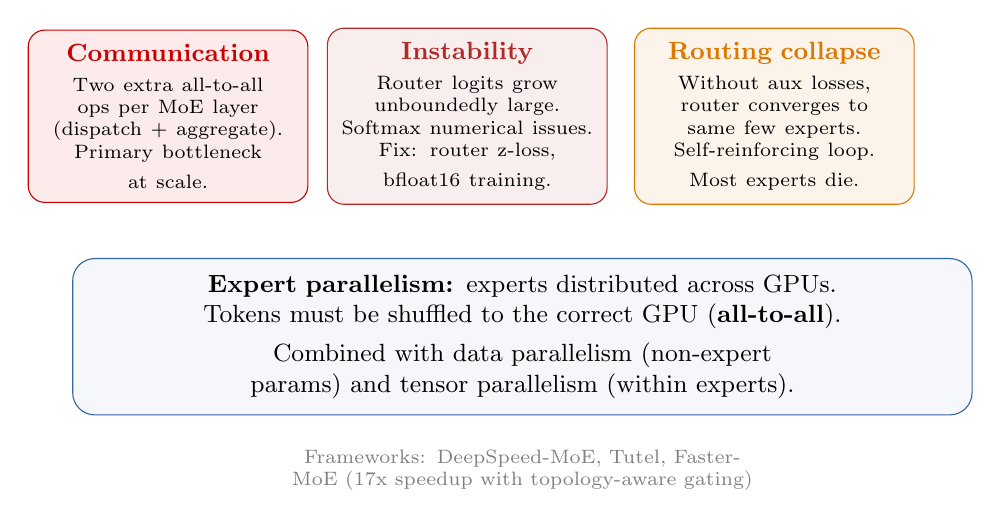
\begin{tikzpicture}
  % Communication
  \node[draw=sampred, fill=sampred!8, rounded corners=6pt, text width=3.2cm, align=center, inner sep=5pt, font=\small] at (-4.5, 2) {
    \textbf{\textcolor{sampred}{Communication}}\\[3pt]
    {\scriptsize Two extra all-to-all\\ops per MoE layer\\(dispatch + aggregate).\\Primary bottleneck\\at scale.}
  };

  % Instability
  \node[draw=warnred, fill=warnred!8, rounded corners=6pt, text width=3.2cm, align=center, inner sep=5pt, font=\small] at (-0.7, 2) {
    \textbf{\textcolor{warnred}{Instability}}\\[3pt]
    {\scriptsize Router logits grow\\unboundedly large.\\Softmax numerical issues.\\Fix: router z-loss,\\bfloat16 training.}
  };

  % Routing collapse
  \node[draw=orange1, fill=orange1!8, rounded corners=6pt, text width=3.2cm, align=center, inner sep=5pt, font=\small] at (3.2, 2) {
    \textbf{\textcolor{orange1}{Routing collapse}}\\[3pt]
    {\scriptsize Without aux losses,\\router converges to\\same few experts.\\Self-reinforcing loop.\\Most experts die.}
  };

  % Expert parallelism
  \node[draw=popblue, fill=popblue!5, rounded corners=8pt, text width=11cm, align=center, inner sep=6pt, font=\small] at (0, -0.8) {
    \textbf{Expert parallelism:} experts distributed across GPUs.\\
    Tokens must be shuffled to the correct GPU (\textbf{all-to-all}).\\[3pt]
    Combined with data parallelism (non-expert params) and tensor parallelism (within experts).
  };

  % Frameworks
  \node[font=\scriptsize, text=gray, text width=10cm, align=center] at (0, -2.5) {
    Frameworks: DeepSpeed-MoE, Tutel, FasterMoE (17x speedup with topology-aware gating)
  };
\end{tikzpicture}
\end{center}
\end{frame}

% ============================================================
% INFERENCE CHALLENGES
% ============================================================
\begin{frame}
\frametitle{Inference challenges}

\begin{center}
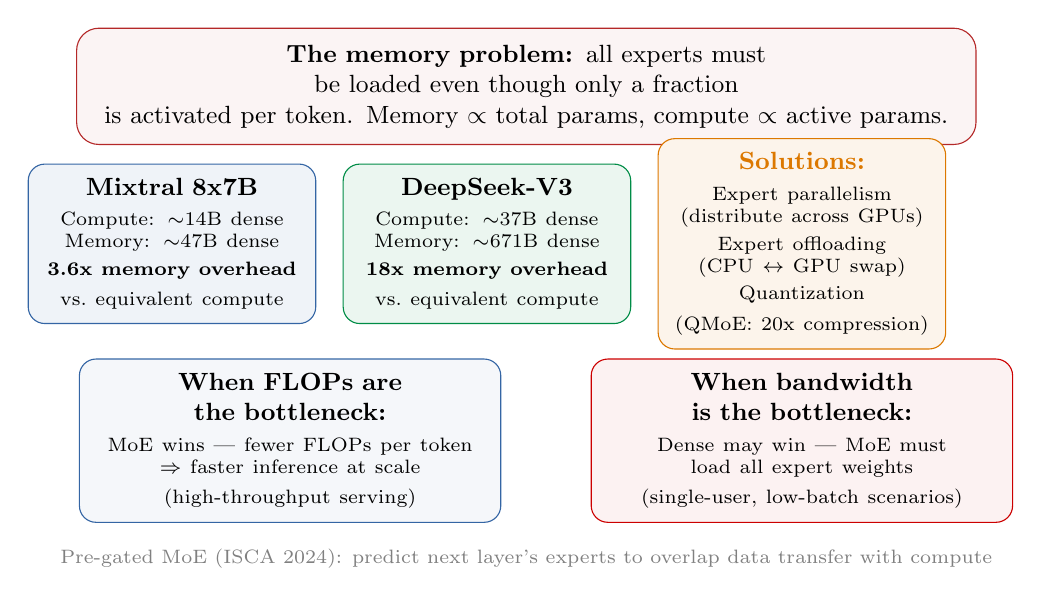
\begin{tikzpicture}
  % The core problem
  \node[draw=warnred, fill=warnred!5, rounded corners=8pt, text width=11cm, align=center, inner sep=6pt, font=\small] at (0, 3) {
    \textbf{The memory problem:} all experts must be loaded even though only a fraction\\
    is activated per token. Memory $\propto$ total params, compute $\propto$ active params.
  };

  % Memory comparison
  \node[draw=popblue, fill=popblue!8, rounded corners=6pt, text width=3.3cm, align=center, inner sep=5pt, font=\small] at (-4.5, 1) {
    \textbf{Mixtral 8x7B}\\[3pt]
    {\scriptsize Compute: $\sim$14B dense\\Memory: $\sim$47B dense\\[2pt]
    \textbf{3.6x memory overhead}\\vs.\ equivalent compute}
  };
  \node[draw=paramgreen, fill=paramgreen!8, rounded corners=6pt, text width=3.3cm, align=center, inner sep=5pt, font=\small] at (-0.5, 1) {
    \textbf{DeepSeek-V3}\\[3pt]
    {\scriptsize Compute: $\sim$37B dense\\Memory: $\sim$671B dense\\[2pt]
    \textbf{18x memory overhead}\\vs.\ equivalent compute}
  };

  % Solutions
  \node[draw=orange1, fill=orange1!8, rounded corners=6pt, text width=3.3cm, align=center, inner sep=5pt, font=\small] at (3.5, 1) {
    \textbf{\textcolor{orange1}{Solutions:}}\\[3pt]
    {\scriptsize Expert parallelism\\(distribute across GPUs)\\[2pt]
    Expert offloading\\(CPU $\leftrightarrow$ GPU swap)\\[2pt]
    Quantization\\(QMoE: 20x compression)}
  };

  % Latency
  \node[draw=popblue, fill=popblue!5, rounded corners=6pt, text width=5cm, align=center, inner sep=5pt, font=\small] at (-3, -1.5) {
    \textbf{When FLOPs are the bottleneck:}\\[3pt]
    {\scriptsize MoE wins --- fewer FLOPs per token\\$\Rightarrow$ faster inference at scale\\(high-throughput serving)}
  };
  \node[draw=sampred, fill=sampred!5, rounded corners=6pt, text width=5cm, align=center, inner sep=5pt, font=\small] at (3.5, -1.5) {
    \textbf{When bandwidth is the bottleneck:}\\[3pt]
    {\scriptsize Dense may win --- MoE must\\load all expert weights\\(single-user, low-batch scenarios)}
  };

  \node[font=\scriptsize, text=gray] at (0, -3) {Pre-gated MoE (ISCA 2024): predict next layer's experts to overlap data transfer with compute};
\end{tikzpicture}
\end{center}
\end{frame}

% ============================================================
% MOE AND SCALING
% ============================================================
\begin{frame}
\frametitle{MoE and scaling laws}

\begin{center}
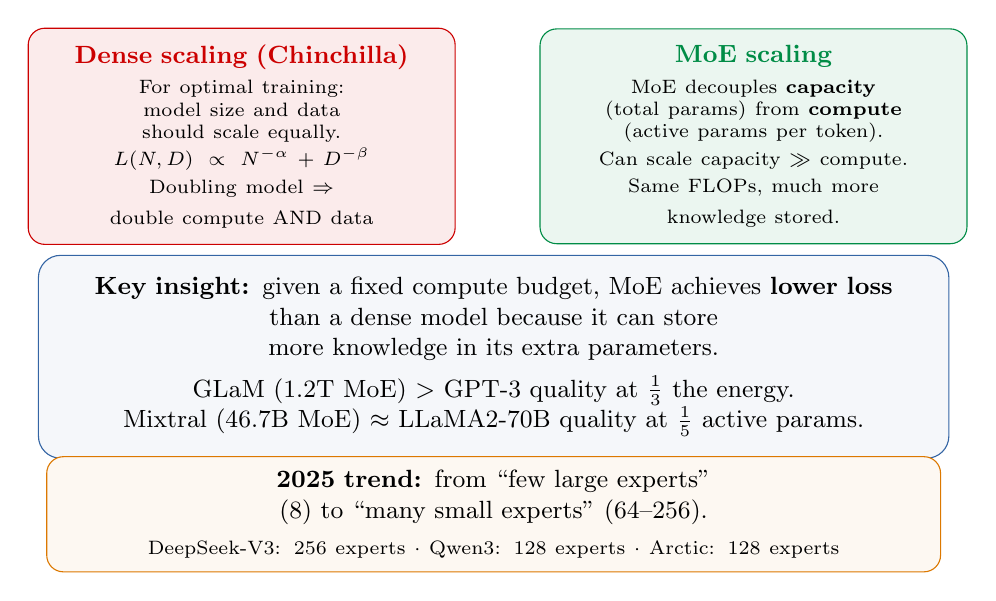
\begin{tikzpicture}
  % Dense scaling
  \node[draw=sampred, fill=sampred!8, rounded corners=6pt, text width=5cm, align=center, inner sep=6pt, font=\small] at (-3, 2.5) {
    \textbf{\textcolor{sampred}{Dense scaling (Chinchilla)}}\\[3pt]
    {\scriptsize For optimal training:\\model size and data\\should scale equally.\\[2pt]
    $L(N, D) \propto N^{-\alpha} + D^{-\beta}$\\[2pt]
    Doubling model $\Rightarrow$\\double compute AND data}
  };

  % MoE scaling
  \node[draw=paramgreen, fill=paramgreen!8, rounded corners=6pt, text width=5cm, align=center, inner sep=6pt, font=\small] at (3.5, 2.5) {
    \textbf{\textcolor{paramgreen}{MoE scaling}}\\[3pt]
    {\scriptsize MoE decouples \textbf{capacity}\\(total params) from \textbf{compute}\\(active params per token).\\[2pt]
    Can scale capacity $\gg$ compute.\\[2pt]
    Same FLOPs, much more\\knowledge stored.}
  };

  % The key insight
  \node[draw=popblue, fill=popblue!5, rounded corners=8pt, text width=11cm, align=center, inner sep=8pt, font=\small] at (0.2, -0.3) {
    \textbf{Key insight:} given a fixed compute budget, MoE achieves \textbf{lower loss}\\
    than a dense model because it can store more knowledge in its extra parameters.\\[4pt]
    GLaM (1.2T MoE) $>$ GPT-3 quality at $\frac{1}{3}$ the energy.\\
    Mixtral (46.7B MoE) $\approx$ LLaMA2-70B quality at $\frac{1}{5}$ active params.
  };

  % Trend
  \node[draw=orange1, fill=orange1!5, rounded corners=6pt, text width=11cm, align=center, inner sep=5pt, font=\small] at (0.2, -2.3) {
    \textbf{2025 trend:} from ``few large experts'' (8) to ``many small experts'' (64--256).\\[2pt]
    {\scriptsize DeepSeek-V3: 256 experts $\cdot$ Qwen3: 128 experts $\cdot$ Arctic: 128 experts}
  };
\end{tikzpicture}
\end{center}
\end{frame}

% ============================================================
% THE FULL LANDSCAPE
% ============================================================
\begin{frame}
\frametitle{The MoE landscape}

\vspace{-0.3cm}
\begin{center}
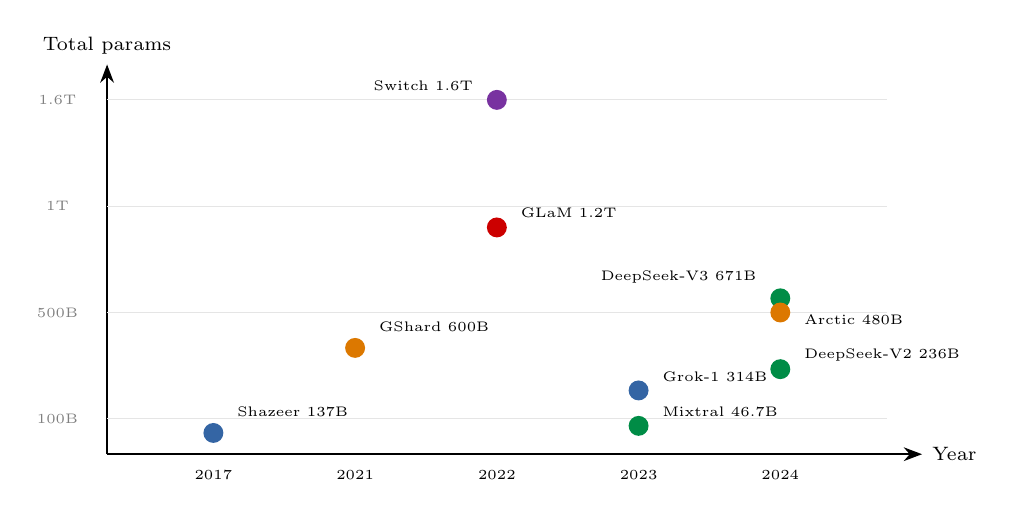
\begin{tikzpicture}[scale=0.9]
  % Axes
  \draw[-Stealth, thick] (-5.5, -2) -- (-5.5, 3.5) node[above, font=\scriptsize] {Total params};
  \draw[-Stealth, thick] (-5.5, -2) -- (6, -2) node[right, font=\scriptsize] {Year};

  % Year labels
  \node[font=\tiny] at (-4, -2.3) {2017};
  \node[font=\tiny] at (-2, -2.3) {2021};
  \node[font=\tiny] at (0, -2.3) {2022};
  \node[font=\tiny] at (2, -2.3) {2023};
  \node[font=\tiny] at (4, -2.3) {2024};

  % Param scale labels
  \node[font=\tiny, text=gray] at (-6.2, -1.5) {100B};
  \node[font=\tiny, text=gray] at (-6.2, 0) {500B};
  \node[font=\tiny, text=gray] at (-6.2, 1.5) {1T};
  \node[font=\tiny, text=gray] at (-6.2, 3) {1.6T};

  % Grid
  \draw[gray!20] (-5.5, -1.5) -- (5.5, -1.5);
  \draw[gray!20] (-5.5, 0) -- (5.5, 0);
  \draw[gray!20] (-5.5, 1.5) -- (5.5, 1.5);
  \draw[gray!20] (-5.5, 3) -- (5.5, 3);

  % Models as dots
  \fill[popblue] (-4, -1.7) circle (4pt);
  \node[font=\tiny, anchor=west] at (-3.8, -1.4) {Shazeer 137B};

  \fill[orange1] (-2, -0.5) circle (4pt);
  \node[font=\tiny, anchor=west] at (-1.8, -0.2) {GShard 600B};

  \fill[violet1] (0, 3) circle (4pt);
  \node[font=\tiny, anchor=east] at (-0.2, 3.2) {Switch 1.6T};

  \fill[sampred] (0, 1.2) circle (4pt);
  \node[font=\tiny, anchor=west] at (0.2, 1.4) {GLaM 1.2T};

  \fill[paramgreen] (2, -1.6) circle (4pt);
  \node[font=\tiny, anchor=west] at (2.2, -1.4) {Mixtral 46.7B};

  \fill[popblue] (2, -1.1) circle (4pt);
  \node[font=\tiny, anchor=west] at (2.2, -0.9) {Grok-1 314B};

  \fill[paramgreen] (4, -0.8) circle (4pt);
  \node[font=\tiny, anchor=west] at (4.2, -0.6) {DeepSeek-V2 236B};

  \fill[paramgreen] (4, 0.2) circle (4pt);
  \node[font=\tiny, anchor=east] at (3.8, 0.5) {DeepSeek-V3 671B};

  \fill[orange1] (4, 0) circle (4pt);
  \node[font=\tiny, anchor=west] at (4.2, -0.1) {Arctic 480B};
\end{tikzpicture}
\end{center}
\end{frame}

% ============================================================
% DEEPSEEK-V3
% ============================================================
\begin{frame}
\frametitle{Case study: DeepSeek-V3}

\begin{center}
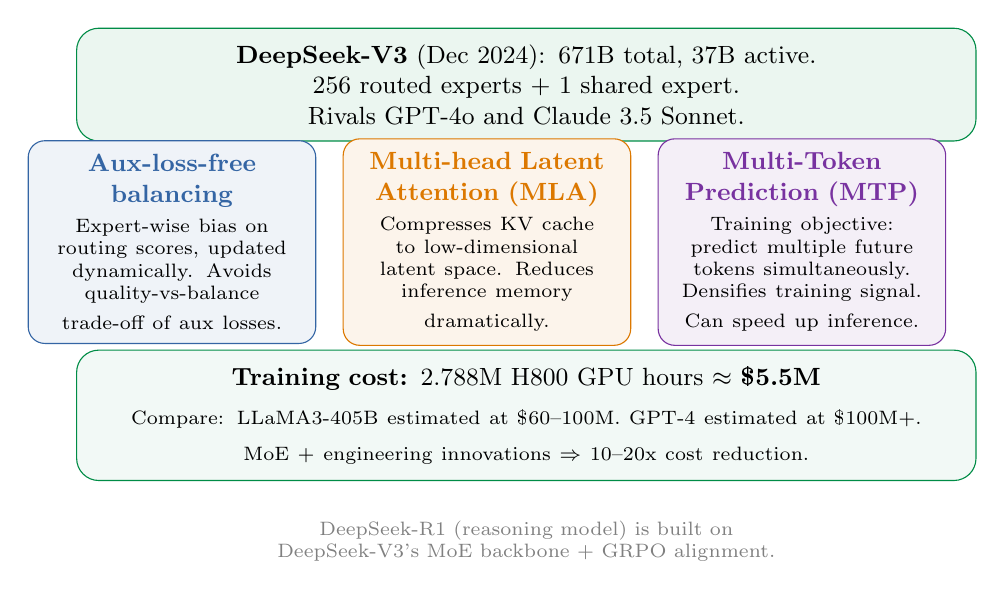
\begin{tikzpicture}
  % Header
  \node[draw=paramgreen, fill=paramgreen!8, rounded corners=8pt, text width=11cm, align=center, inner sep=6pt, font=\small] at (0, 3) {
    \textbf{DeepSeek-V3} (Dec 2024): 671B total, 37B active.\\
    256 routed experts + 1 shared expert. Rivals GPT-4o and Claude 3.5 Sonnet.
  };

  % Three innovations
  \node[draw=popblue, fill=popblue!8, rounded corners=6pt, text width=3.3cm, align=center, inner sep=5pt, font=\small] at (-4.5, 1) {
    \textbf{\textcolor{popblue}{Aux-loss-free\\balancing}}\\[3pt]
    {\scriptsize Expert-wise bias on\\routing scores, updated\\dynamically. Avoids\\quality-vs-balance\\trade-off of aux losses.}
  };

  \node[draw=orange1, fill=orange1!8, rounded corners=6pt, text width=3.3cm, align=center, inner sep=5pt, font=\small] at (-0.5, 1) {
    \textbf{\textcolor{orange1}{Multi-head Latent\\Attention (MLA)}}\\[3pt]
    {\scriptsize Compresses KV cache\\to low-dimensional\\latent space. Reduces\\inference memory\\dramatically.}
  };

  \node[draw=violet1, fill=violet1!8, rounded corners=6pt, text width=3.3cm, align=center, inner sep=5pt, font=\small] at (3.5, 1) {
    \textbf{\textcolor{violet1}{Multi-Token\\Prediction (MTP)}}\\[3pt]
    {\scriptsize Training objective:\\predict multiple future\\tokens simultaneously.\\Densifies training signal.\\Can speed up inference.}
  };

  % Cost
  \node[draw=paramgreen, fill=paramgreen!5, rounded corners=8pt, text width=11cm, align=center, inner sep=6pt, font=\small] at (0, -1.2) {
    \textbf{Training cost:} 2.788M H800 GPU hours $\approx$ \textbf{\$5.5M}\\[3pt]
    {\scriptsize Compare: LLaMA3-405B estimated at \$60--100M. GPT-4 estimated at \$100M+.}\\[2pt]
    {\scriptsize MoE + engineering innovations $\Rightarrow$ 10--20x cost reduction.}
  };

  % DeepSeek-R1
  \node[font=\scriptsize, text=gray, text width=10cm, align=center] at (0, -2.8) {
    DeepSeek-R1 (reasoning model) is built on DeepSeek-V3's MoE backbone + GRPO alignment.
  };
\end{tikzpicture}
\end{center}
\end{frame}

% ============================================================
% PRACTICAL GUIDE
% ============================================================
\begin{frame}
\frametitle{Practical guide}

\begin{center}
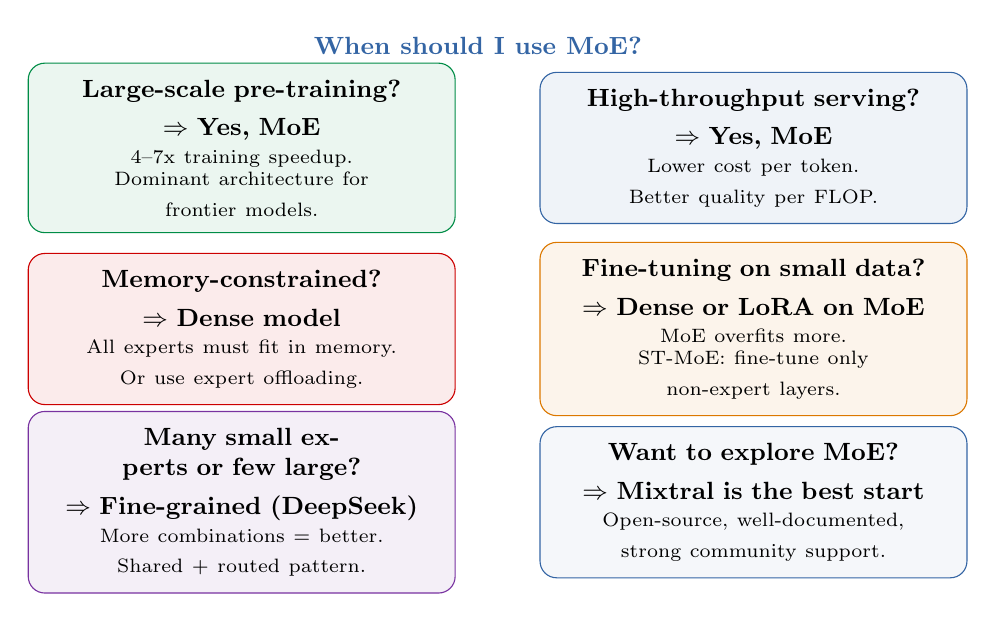
\begin{tikzpicture}
  \node[font=\small\bfseries, text=popblue] at (0, 3.3) {When should I use MoE?};

  % Decision boxes
  \node[draw=paramgreen, fill=paramgreen!8, rounded corners=6pt, text width=5cm, align=center, inner sep=6pt, font=\small] at (-3, 2) {
    \textbf{Large-scale pre-training?}\\[3pt]
    $\Rightarrow$ \textbf{Yes, MoE}\\[2pt]
    {\scriptsize 4--7x training speedup.\\Dominant architecture for\\frontier models.}
  };
  \node[draw=popblue, fill=popblue!8, rounded corners=6pt, text width=5cm, align=center, inner sep=6pt, font=\small] at (3.5, 2) {
    \textbf{High-throughput serving?}\\[3pt]
    $\Rightarrow$ \textbf{Yes, MoE}\\[2pt]
    {\scriptsize Lower cost per token.\\Better quality per FLOP.}
  };
  \node[draw=sampred, fill=sampred!8, rounded corners=6pt, text width=5cm, align=center, inner sep=6pt, font=\small] at (-3, -0.3) {
    \textbf{Memory-constrained?}\\[3pt]
    $\Rightarrow$ \textbf{Dense model}\\[2pt]
    {\scriptsize All experts must fit in memory.\\Or use expert offloading.}
  };
  \node[draw=orange1, fill=orange1!8, rounded corners=6pt, text width=5cm, align=center, inner sep=6pt, font=\small] at (3.5, -0.3) {
    \textbf{Fine-tuning on small data?}\\[3pt]
    $\Rightarrow$ \textbf{Dense or LoRA on MoE}\\[2pt]
    {\scriptsize MoE overfits more.\\ST-MoE: fine-tune only\\non-expert layers.}
  };
  \node[draw=violet1, fill=violet1!8, rounded corners=6pt, text width=5cm, align=center, inner sep=6pt, font=\small] at (-3, -2.5) {
    \textbf{Many small experts or few large?}\\[3pt]
    $\Rightarrow$ \textbf{Fine-grained (DeepSeek)}\\[2pt]
    {\scriptsize More combinations = better.\\Shared + routed pattern.}
  };
  \node[draw=popblue, fill=popblue!5, rounded corners=6pt, text width=5cm, align=center, inner sep=6pt, font=\small] at (3.5, -2.5) {
    \textbf{Want to explore MoE?}\\[3pt]
    $\Rightarrow$ \textbf{Mixtral is the best start}\\[2pt]
    {\scriptsize Open-source, well-documented,\\strong community support.}
  };
\end{tikzpicture}
\end{center}
\end{frame}

% ============================================================
% QUESTIONS
% ============================================================
\begin{frame}
\begin{center}
\vspace{2cm}
{\Huge \textcolor{popblue}{Questions?}}

\vspace{1cm}
{\normalsize All DL4NLP topics complete!}
\end{center}
\end{frame}

\end{document}
